\documentclass[border=6pt]{standalone}
\usepackage[T1]{fontenc}
\usepackage{amsmath,amssymb}
\usepackage{tikz}
\usetikzlibrary{arrows.meta,positioning,fit,backgrounds,calc}

\definecolor{cBlue}{HTML}{3C7EC2}
\definecolor{cRed}{HTML}{CC4444}
\definecolor{cOrange}{HTML}{E8873D}
\definecolor{cGreen}{HTML}{4EA84E}
\definecolor{cGray}{HTML}{5F6B7A}

\begin{document}
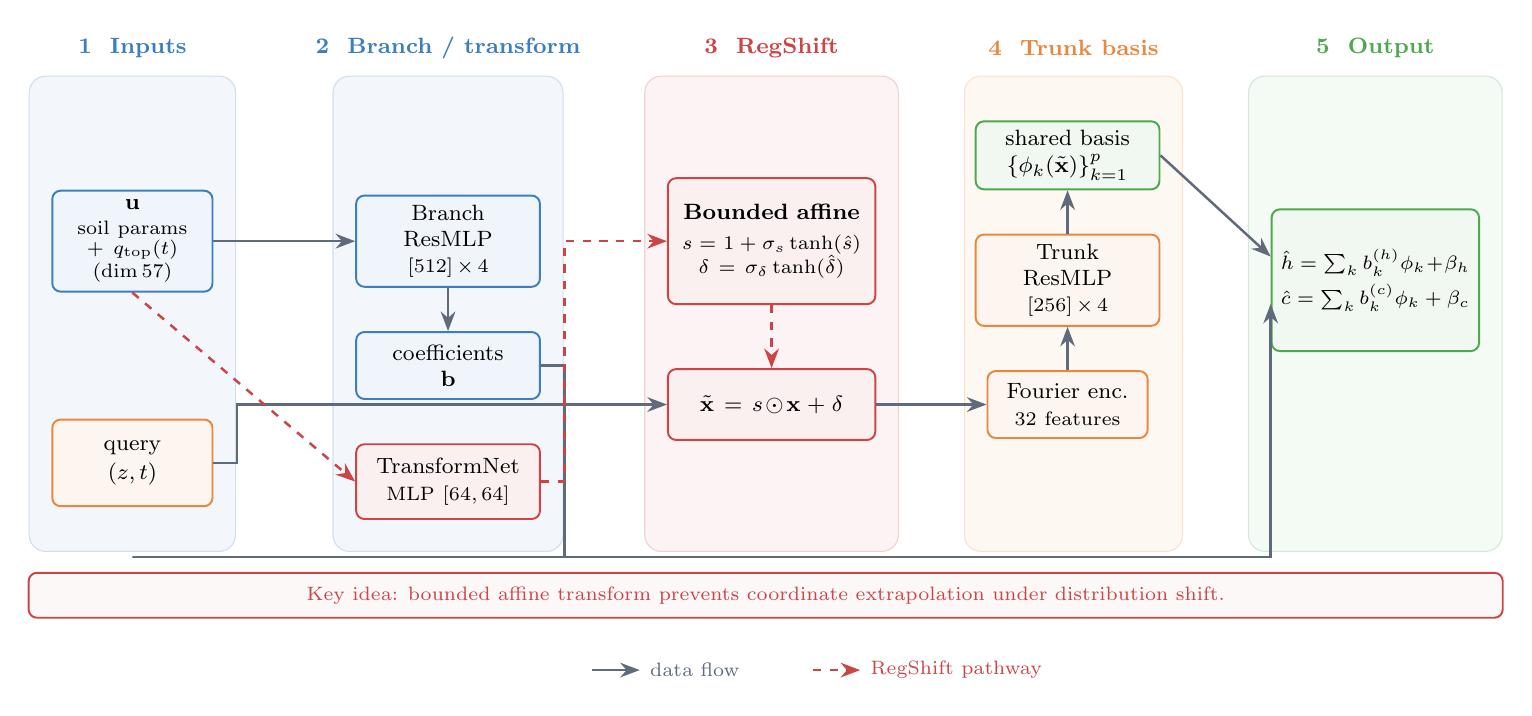
\begin{tikzpicture}[
  >=Stealth,
  font=\footnotesize,
  node distance=0.6cm and 0.8cm,
  box/.style={draw=#1, fill=#1!8, rounded corners=3pt,
              minimum height=1.1cm, align=center, text width=2.1cm,
              line width=0.7pt},
  smallbox/.style={draw=#1, fill=#1!8, rounded corners=3pt,
              minimum height=0.85cm, align=center, text width=1.8cm,
              line width=0.7pt},
  arr/.style={->, line width=0.9pt, color=cGray},
  redarr/.style={->, line width=0.9pt, color=cRed, dashed},
]

% ---- Stage 1: Inputs ----
\node[box=cBlue, text width=1.8cm] (ubox)
  {$\mathbf{u}$\\[1pt]\scriptsize soil params\\[-1pt]\scriptsize $+ \; q_{\mathrm{top}}(t)$\\[-1pt]\scriptsize (dim\,57)};

\node[box=cOrange, text width=1.8cm, below=1.6cm of ubox] (qbox)
  {query\\[1pt]$(z,t)$};

% ---- Stage 2: Branch / Transform ----
\node[box=cBlue, right=1.8cm of ubox] (branch)
  {Branch\\ResMLP\\\scriptsize $[512]\!\times\!4$};

\node[box=cBlue, below=0.55cm of branch, minimum height=0.85cm] (coeffs)
  {coefficients\\$\mathbf{b}$};

\node[box=cRed, below=0.55cm of coeffs, minimum height=0.95cm] (tnet)
  {TransformNet\\\scriptsize MLP $[64,64]$};

% ---- Stage 3: RegShift ----
\node[box=cRed, right=1.6cm of branch, text width=2.4cm, minimum height=1.6cm] (affine)
  {\textbf{Bounded affine}\\[3pt]
   \scriptsize $s = 1+\sigma_s\tanh(\hat{s})$\\[-1pt]
   \scriptsize $\delta = \sigma_\delta\tanh(\hat{\delta})$};

\node[box=cRed, below=0.8cm of affine, minimum height=0.9cm, text width=2.4cm] (xmap)
  {$\tilde{\mathbf{x}} = s\!\odot\!\mathbf{x} + \delta$};

% ---- Stage 4: Trunk ----
\node[smallbox=cOrange, right=1.4cm of xmap] (fourier)
  {Fourier enc.\\\scriptsize 32 features};

\node[box=cOrange, above=0.55cm of fourier, minimum height=0.9cm] (trunk)
  {Trunk\\ResMLP\\\scriptsize $[256]\!\times\!4$};

\node[box=cGreen, above=0.55cm of trunk, minimum height=0.85cm] (basis)
  {shared basis\\$\{\phi_k(\tilde{\mathbf{x}})\}_{k=1}^{p}$};

% ---- Stage 5: Output ----
\node[box=cGreen, right=1.4cm of trunk, text width=2.4cm, minimum height=1.8cm] (out)
  {\scriptsize $\hat{h} = \sum_k b^{(h)}_k\phi_k + \beta_h$\\[2pt]
   \scriptsize $\hat{c} = \sum_k b^{(c)}_k\phi_k + \beta_c$};

% ---- Shared label positions ----
\coordinate (phi-label-pos) at ($(basis.east)!0.5!([yshift=0.3cm]out.west)$);

% ---- Background stages (uniform height) ----
\coordinate (stage-top) at ([yshift=8pt]basis.north);
\coordinate (stage-bot) at ([yshift=-8pt]qbox.south);

\begin{scope}[on background layer]
  \node[fit={(ubox.west |- stage-top)(qbox.south -| ubox.east)(ubox.west |- stage-bot)},
        fill=cBlue!6, draw=cBlue!25, rounded corners=6pt, inner sep=8pt] (bg1) {};
  \node[fit={(branch.west |- stage-top)(tnet.south -| branch.east)(branch.west |- stage-bot)},
        fill=cBlue!6, draw=cBlue!25, rounded corners=6pt, inner sep=8pt] (bg2) {};
  \node[fit={(affine.west |- stage-top)(xmap.south -| affine.east)(affine.west |- stage-bot)},
        fill=cRed!6, draw=cRed!25, rounded corners=6pt, inner sep=8pt] (bg3) {};
  \node[fit={(fourier.west |- stage-top)(fourier.south -| trunk.east)(fourier.west |- stage-bot)},
        fill=cOrange!6, draw=cOrange!25, rounded corners=6pt, inner sep=8pt] (bg4) {};
  \node[fit={(out.west |- stage-top)(out.south -| out.east)(out.west |- stage-bot)},
        fill=cGreen!6, draw=cGreen!25, rounded corners=6pt, inner sep=8pt] (bg5) {};
\end{scope}

% ---- Stage labels (aligned at a single y-coordinate) ----
\coordinate (label-y) at ([yshift=0.35cm]bg1.north);
\node[font=\footnotesize\bfseries, text=cBlue]   at (bg1 |- label-y) {1~~Inputs};
\node[font=\footnotesize\bfseries, text=cBlue]   at (bg2 |- label-y) {2~~Branch / transform};
\node[font=\footnotesize\bfseries, text=cRed]    at (bg3 |- label-y) {3~~RegShift};
\node[font=\footnotesize\bfseries, text=cOrange] at (bg4 |- label-y) {4~~Trunk basis};
\node[font=\footnotesize\bfseries, text=cGreen]  at (bg5 |- label-y) {5~~Output};

% ---- Arrows: sample-descriptor path ----
\draw[arr] (ubox) -- (branch);
\draw[arr] (branch) -- (coeffs);

% b_k → Output: route below stages 3-4, enter output left side (lower)
\coordinate (b-route-bot) at ($(stage-bot)-(0, 0.35cm)$);
\coordinate (b-route-left) at ([xshift=0.3cm]coeffs.east |- b-route-bot);
\coordinate (b-route-right) at ([xshift=-0.3cm]out.west |- b-route-bot);
\coordinate (b-label-pos) at (b-route-bot -| phi-label-pos);
\coordinate (b-gap-left) at ([xshift=-0.18cm]b-label-pos);
\coordinate (b-gap-right) at ([xshift=0.18cm]b-label-pos);
\draw[arr] (coeffs.east) -- ++(0.3, 0)
  |- (b-route-bot) -| ([yshift=-0.3cm]out.west);

% ---- Arrows: query path ----
\draw[arr] (qbox.east) -- ++(0.3,0) |- (xmap.west);
\draw[arr] (xmap) -- (fourier);
\draw[arr] (fourier) -- (trunk);
\draw[arr] (trunk) -- (basis);

% φ_k → Output: from basis into output left side (upper)
\draw[arr] (basis.east) -- ([yshift=0.3cm]out.west);

% ---- Arrows: RegShift-specific (dashed red) ----
\draw[redarr] (ubox.south) -- (tnet.west);
\draw[redarr] (tnet.east) -- ++(0.3,0) |- (affine.west);
\draw[redarr] (affine) -- (xmap);

% ---- Path labels removed to avoid left-edge overflow (redundant with stage labels) ----

% ---- Key-idea banner spanning full width ----
\path let \p1=(bg1.west), \p2=(bg5.east), \n1={\x2-\x1} in
  node[draw=cRed, fill=cRed!4, rounded corners=3pt, line width=0.7pt,
       font=\scriptsize, align=center, text=cRed,
       inner xsep=0pt, inner ysep=5pt,
       minimum width=\n1]
  at ([yshift=-0.55cm]bg1.south -| {$(bg1.west)!0.5!(bg5.east)$})
  {Key idea: bounded affine transform prevents
   coordinate extrapolation under distribution shift.};

% ---- Legend (centered below key-idea banner) ----
\path let \p1=(bg1.west), \p2=(bg5.east) in
  coordinate (leg-center) at ({0.5*\x1+0.5*\x2}, \y1);
\coordinate (leg-y) at ([yshift=-1.5cm]bg1.south);
\draw[arr] ([xshift=-2.2cm]leg-center |- leg-y) -- ++(0.6,0)
  node[right, font=\scriptsize, text=cGray] {data flow};
\draw[redarr] ([xshift=0.6cm]leg-center |- leg-y) -- ++(0.6,0)
  node[right, font=\scriptsize, text=cRed] {RegShift pathway};

\end{tikzpicture}
\end{document}
